%-------------------------------
%	DOCUMENT SETTINGS
%-------------------------------
\documentclass[a4paper]{article}

\setlength{\hoffset}{-3.2cm}
\setlength{\voffset}{-3cm}
\setlength{\textwidth}{18.7cm}
\setlength{\textheight}{25.5cm}
\setlength{\parskip}{0pt}
\setlength{\parindent}{0in}

%----------------------------------------------------------------------------------------
%	PACKAGES AND OTHER DOCUMENT CONFIGURATIONS
%----------------------------------------------------------------------------------------

\usepackage{mathtools}
\usepackage{dsfont}
\usepackage[shortlabels]{enumitem}
\DeclarePairedDelimiter\abs{\lvert}{\rvert}%
\usepackage{cancel}
\usepackage{blindtext} % Package to generate dummy text
\usepackage{charter} % Use the Charter font
\usepackage[utf8]{inputenc} % Use UTF-8 encoding
\usepackage{microtype} % Slightly tweak font spacing for aesthetics
\usepackage[english]{babel} % Language hyphenation and typographical rules
\usepackage{amsthm, amsmath, amssymb} % Mathematical typesetting
\usepackage{float} % Improved interface for floating objects
\usepackage[final, colorlinks = true, 
linkcolor = black, 
citecolor = black]{hyperref} % For hyperlinks in the PDF
\usepackage{graphicx, multicol} % Enhanced support for graphics
\usepackage{xcolor} % Driver-independent color extensions
\usepackage{marvosym, wasysym} % More symbols
\usepackage{rotating} % Rotation tools
\usepackage{censor} % Facilities for controlling restricted text
\usepackage{listings} % Environment for non-formatted code, !uses style file!
\usepackage{pseudocode} % Environment for specifying algorithms in a natural way
% Environment for f-structures, !uses style file!
\usepackage{booktabs} % Enhances quality of tables
\usepackage{tikz-qtree} % Easy tree drawing tool
% Configuration for b-trees and b+-trees, !uses style file!
%\usepackage[backend=biber,style=numeric,
%            sorting=nyt]{biblatex} % Complete reimplementation of bibliographic facilities
%\addbibresource{ecl.bib}
\usepackage{csquotes} % Context sensitive quotation facilities
\usepackage[yyyymmdd]{datetime} % Uses YEAR-MONTH-DAY format for dates
\renewcommand{\dateseparator}{-} % Sets dateseparator to '-'
\usepackage{fancyhdr} % Headers and footers
\pagestyle{fancy} % All pages have headers and footers
\fancyhead{}\renewcommand{\headrulewidth}{0pt} % Blank out the default header
\fancyfoot[L]{} % Custom footer text
\fancyfoot[C]{} % Custom footer text
\fancyfoot[R]{\thepage} % Custom footer text
\newcommand{\note}[1]{\marginpar{\scriptsize \textcolor{red}{#1}}} % Enables comments in red on margin

%----------------------------------------------------------------------------------------
%	CUSTOM COMMANDS
%----------------------------------------------------------------------------------------

\newcommand{\R}{\mathbb{R}}
\newcommand{\E}{\mathbb{E}}
\newcommand{\I}{\mathbb{I}}
\newcommand{\Var}{\text{Var}}
% Para poner sonrisa sobre puntos suspensivos. Uso: \overplace{n}{\dotsc}
\newcommand{\overplace}[2]{%
	\overset{\substack{#1\\\smile}}{#2}%
}

\begin{document}
	
%-------------------------------
%	TITLE SECTION
%-------------------------------

\fancyhead[C]{}
\hrule \medskip % Upper rule
\begin{minipage}{0.295\textwidth} 
	\raggedright
	\footnotesize
	José Antonio Álvarez Ocete \hfill\\   
	77553417Q \hfill\\
	joseantonio.alvarezo@estudiante.uam.es
\end{minipage}
\begin{minipage}{0.4\textwidth} 
	\centering 
	\large 
	Entrega de problemas Boostrap\\ 
	\normalsize 
	Métodos Avanzados en Estadística\\ 
\end{minipage}
\begin{minipage}{0.295\textwidth} 
	\raggedleft
	\today\hfill\\
\end{minipage}
\medskip\hrule 
\bigskip

%-------------------------------
%	CONTENTS
%-------------------------------

\section*{Ejercicio 6.}

\textbf{Enunciado.} Sean $X_1, \ldots, X_n$ variables aleatorias \emph{i.i.d.} de una distribución con densidad $f$. Se considera el estimador del núcleo $\hat f$ con núcleo rectangular $K(x) = \I_{[-1/2,1/2]}(x)$ y parámetro de suavizado $h$.

\begin{enumerate}[a)]
	\item Calcula el sesgo y la varianza de $\hat f(x)$, para un valor de $x$ fijo.
	
	\item Demuestra que tanto el sesgo como la varianza tienden a cero si $h \rightarrow 0$ y $nh \rightarrow \infty$.
\end{enumerate}

Al estudiar el sesgo y la varianza de $\hat f(x)$ para un valor de $x$ fijo, estudiamos dichos valores respecto a la muestra tomada de  $X_1, \ldots, X_n$. En primer lugar, calculemos la esperanza del núcleo rectangular dado por la función indicatriz:

\[
	\E \bigg[ K\bigg(\frac{x - t}{h}\bigg) \bigg] = \int_{-\infty}^{+\infty} f(t) \; K\bigg(\frac{x - t}{h}\bigg) \; dt 
\]

Utilizamos el cambio de variable $w = \frac{x-t}{h}, dw = -\frac{dt}{h}$ e invirtiendo los límites de integración obtenemos:

\begin{align}
	\label{eq-nucleo}
	\begin{split}
		\E \bigg[ K\bigg(\frac{x - t}{h}\bigg) \bigg] & = \int_{-\infty}^{+\infty} f(t) \; K\bigg(\frac{x - t}{h}\bigg) \; dt \\
		& = \int_{+\infty}^{-\infty} f(x - wh) \; K(w) \; (-h) \; dw \\
		& = h \int_{-\infty}^{+\infty} f(x - wh) \; \I_{[-1/2,1/2]}(w) \; dw \\
		& = h \int_{-\frac{1}{2}}^{\frac{1}{2}} f(x - wh) dw \\
	\end{split}
\end{align}

Calculemos el sesgo de nuestro estimador del núcleo haciendo uso de la expresión anterior. Para ello calculamos su esperanza:

\begin{align*}
	\E [ \hat f(x)] & = \E \bigg[ \frac{1}{nh} \sum_{i=1}^n K\bigg(\frac{x - t}{h}\bigg) \bigg] \\
	& \stackrel{\text{iid}}{=} \frac{1}{nh} \; n \E \bigg[ K\bigg(\frac{x - t}{h}\bigg) \bigg] \\
	& \stackrel{(\ref{eq-nucleo})}{=} \frac{1}{h} \; h \int_{-\frac{1}{2}}^{\frac{1}{2}} f(x - wh) dw \\
	& = \int_{-\frac{1}{2}}^{\frac{1}{2}} f(x - wh) dw \\
\end{align*}

Este valor únicamente depende del punto fijado $x$, el parámetro de suavizado $h$ y la función de densidad $f$. Su valor equivale al área bajo la gráfica de $f$ en el intervalo $[x - h/2, x + h/2]$, como se puede apreciar en la figura \ref{fig-sesgo}. \\

\begin{figure}[H]
	\centering
	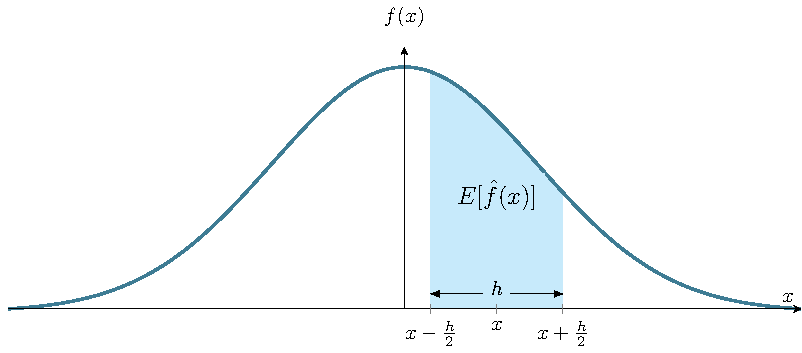
\includegraphics[scale=0.9]{sesgo}
	\caption{Representación gráfica del valor $\E [\hat f(x)]$.}
	\label{fig-sesgo}
\end{figure}

Es decir, estamos aproximando el valor de una función en un punto por su integral en un intervalor centrado en dicho punto. Naturalmente, al tomar $h \rightarrow 0$, dicho valor tiende al valor del punto. Es decir, el sesgo tiende a $0$. Analíticamente:

\begin{align*}
	\text{Sesgo}(f) & = E [ \hat f(x) ] - f(x) \\
	& = \int_{-\frac{1}{2}}^{\frac{1}{2}} f(x - wh) dw - f(x) \\
	& \stackrel{h \rightarrow \infty}{\longrightarrow} \int_{-\frac{1}{2}}^{\frac{1}{2}} f(x) dw - f(x) \\
	& =  f(x) \underbrace{\int_{-\frac{1}{2}}^{\frac{1}{2}} dw}_{= 1} - f(x) \\
	& =  f(x) - f(x) = 0 \\
\end{align*}

Por otro lado, podemos darnos cuenta de lo siguiente:

\begin{equation}
	\label{eq-cuadrado}
	K(x)^2 = K(x) \quad \forall x \in \R,
\end{equation}

pues la función indicatriz tiene por imagen el conjunto $\{0,1\}$ y la función $x \mapsto x^2$ sobre este conjunto es la identidad. Calculemos la varianza del estimador del núcleo:

\begin{align*}
	\Var [ \hat f(x)] & = \Var \bigg[ \frac{1}{nh} \sum_{i=1}^n K\bigg(\frac{x - t}{h}\bigg) \bigg] \\
	& \stackrel{\text{iid}}{=} \frac{1}{n^2 h^2} \; n \Var \bigg[ K\bigg(\frac{x - t}{h}\bigg) \bigg] \\
	& = \frac{1}{n h^2} \bigg( \E \bigg[ K\bigg(\frac{x - t}{h}\bigg)^2 \bigg] - \E \bigg[ K\bigg(\frac{x - t}{h}\bigg) \bigg]^2 \bigg)  \\
	& \stackrel{(\ref{eq-cuadrado})}{=} \frac{1}{n h^2} \bigg( \E \bigg[ K\bigg(\frac{x - t}{h}\bigg) \bigg] - \E \bigg[ K\bigg(\frac{x - t}{h}\bigg) \bigg]^2 \bigg)  \\
	& \stackrel{(\ref{eq-nucleo})}{=} \frac{1}{n h^2} \bigg( h \; \int_{-\frac{1}{2}}^{\frac{1}{2}} f(x - wh) dw - h^2 \; \bigg( \int_{-\frac{1}{2}}^{\frac{1}{2}} f(x - wh) dw\bigg) ^2 \bigg) \\
	& = \frac{1}{n h} \bigg( \int_{-\frac{1}{2}}^{\frac{1}{2}} f(x - wh) dw - h \; \bigg( \int_{-\frac{1}{2}}^{\frac{1}{2}} f(x - wh) dw\bigg) ^2 \bigg) \\
\end{align*}

Finalmente probamos que la varianza tiende a $0$ si $h \rightarrow 0$ y $nh \rightarrow \infty$:

\[
	\Var [ \hat f(x)] = \underbrace{\frac{1}{n h}}_{\hookrightarrow 0} \bigg( \underbrace{\int_{-\frac{1}{2}}^{\frac{1}{2}} f(x - wh) dw}_{\hookrightarrow f(x)} - \underbrace{h \; \bigg( \int_{-\frac{1}{2}}^{\frac{1}{2}} f(x - wh) dw\bigg) ^2}_{\hookrightarrow 0} \bigg)
	\longrightarrow 0
\]

Aunque ya probamos que el error cuadrático medio para un núcleo cualquiera tiende a $0$, en este ejercicio lo hemos probado para el caso del núcleo indicatriz sin el uso de aproximaciones.

\end{document}
